\section{Множество Мандельброта}

\subsection{Реализация}

\begin{lstlisting}[caption=Построение множества Мандельброта]
import numpy as np
import matplotlib.pyplot as plt

class Mandelbrot:
    def __init__(self, width=800, height=800, max_iterations=100, 
                 xmin=-2.0, xmax=1.0, ymin=-1.5, ymax=1.5):
        self.width = width
        self.height = height
        self.max_iterations = max_iterations
        self.xmin = xmin
        self.xmax = xmax
        self.ymin = ymin
        self.ymax = ymax
        
    def compute(self):
        # take a bounded part of the complex plane and construct a grid on it
        x = np.linspace(self.xmin, self.xmax, self.width)
        y = np.linspace(self.ymin, self.ymax, self.height)
        X, Y = np.meshgrid(x, y)
        C = X + 1j * Y
        
        # init arrays
        z = np.zeros_like(C)
        iterations = np.zeros(C.shape, dtype=int)
        
        # construct a sequence iteratively
        for i in range(self.max_iterations + 1):
            mask = np.abs(z) <= 2.0
            z[mask] = z[mask]**2 + C[mask]
            iterations[mask] = i
        
        return iterations
    
    def plot(self, cmap='viridis'):
        iterations = self.compute()
        
        plt.figure(figsize=(10, 10))
        
        # create cmap
        cmap_obj = plt.cm.get_cmap(cmap)
        cmap_obj.set_under('black')
        
        #extent - borders, origin - position (0,0), vmin - scope of visibility for cmap
        plt.imshow(iterations, 
                  extent=[self.xmin, self.xmax, self.ymin, self.ymax],
                  cmap=cmap_obj, 
                  origin='lower',
                  vmin=1,
                  vmax=self.max_iterations)
        
        plt.colorbar(label='Количество')
        plt.xlabel('Re(c)')
        plt.ylabel('Im(c)')
        plt.title(f'Множество Мандельброта (max iterations: {self.max_iterations})')
        plt.show()

# example of a function call
mandel3 = Mandelbrot(
  xmin=-0.75, xmax=-0.65,
  ymin=0.1, ymax=0.2,
  max_iterations=300
)
mandel3.plot()
\end{lstlisting}

\subsection{Примеры визуализации}

\begin{figure}[H]
    \captionsetup[subfigure]{labelformat=empty, justification=centering}
    \centering
    \begin{subfigure}{0.4\textwidth}
        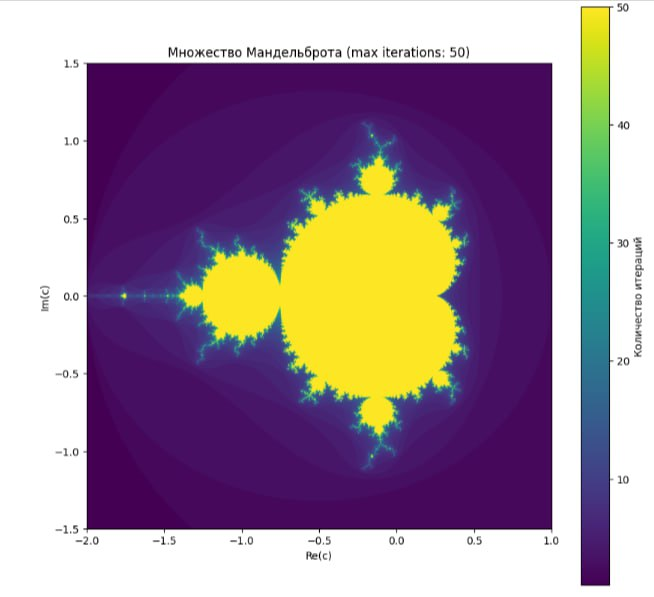
\includegraphics[width=\textwidth]{plots/M1.jpg}
        \caption{Множество Мандельброта, 50~итераций}
    \end{subfigure}
    \hspace{1.7cm}
    \begin{subfigure}{0.4\textwidth}
        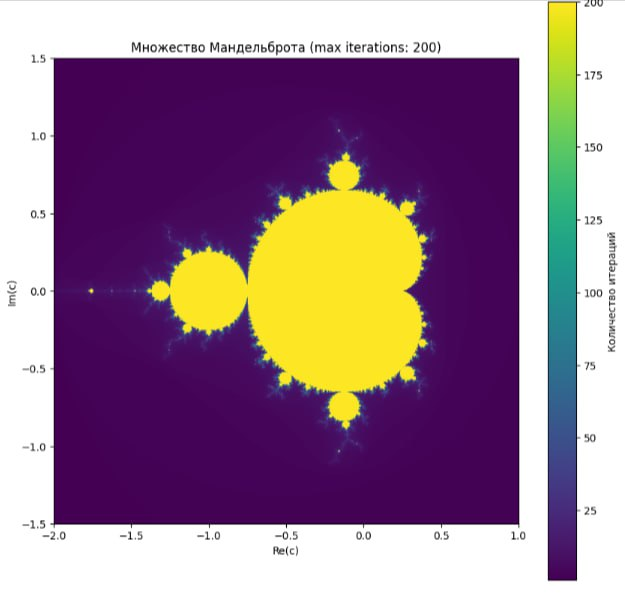
\includegraphics[width=\textwidth]{plots/M2.jpg}
        \caption{Множество Мандельброта, 200~итераций}
    \end{subfigure}
    \\
    \begin{subfigure}{0.4\textwidth}
        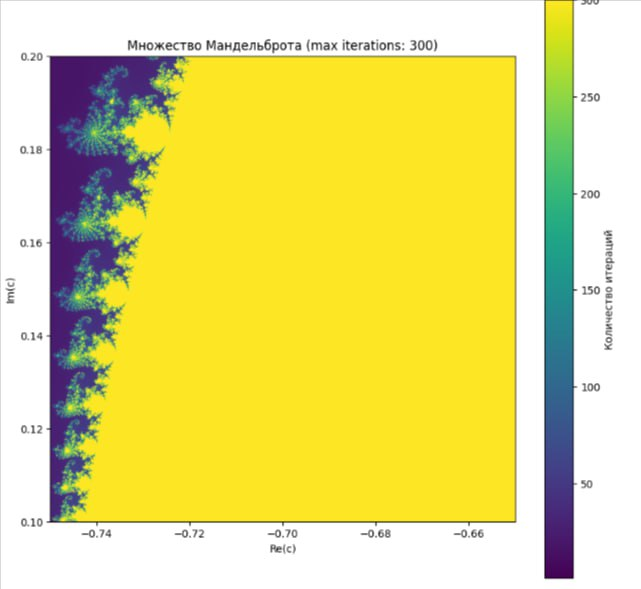
\includegraphics[width=\textwidth]{plots/M3.jpg}
        \caption{Приближение множества Мандельброта, 300 итераций }
    \end{subfigure}
    \hspace{1.7cm}
    \begin{subfigure}{0.4\textwidth}
        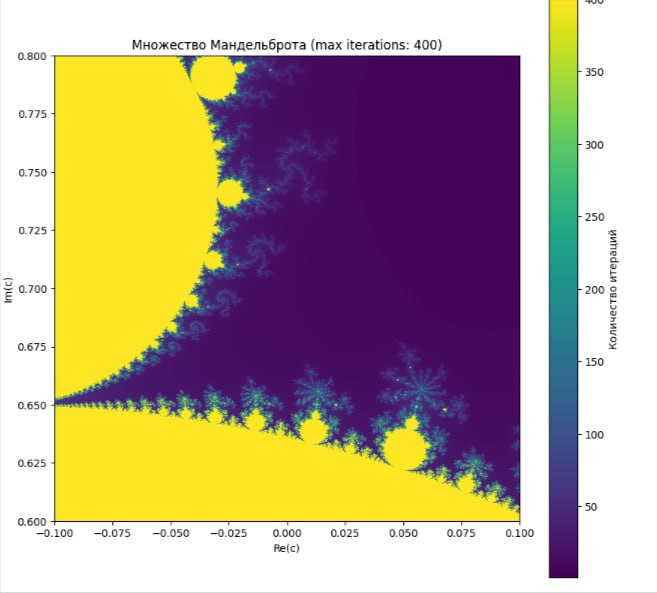
\includegraphics[width=\textwidth]{plots/M4.jpg}
        \caption{Приближение множества Мандельброта на стыке, 400~итераций }
    \end{subfigure}
    \hspace{1.7cm}
    \begin{subfigure}{0.4\textwidth}
        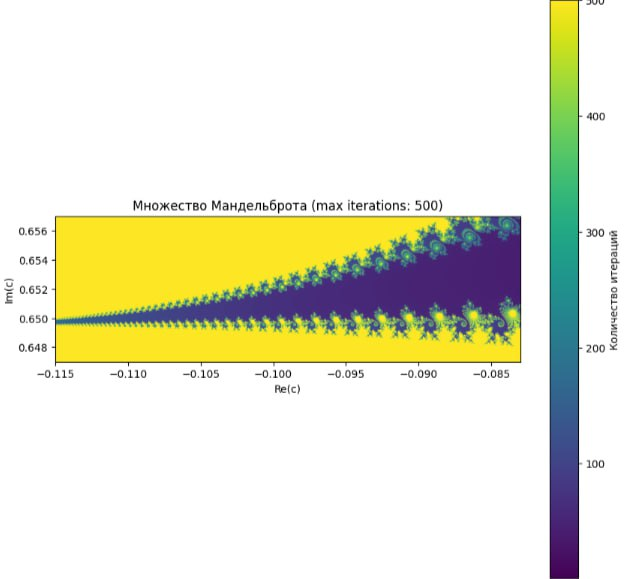
\includegraphics[width=\textwidth]{plots/M5.jpg}
        \caption{Приближение множества Мандельброта по центру слева, 400~итераций }
    \end{subfigure}
    \hspace{1.7cm}
    \begin{subfigure}{0.4\textwidth}
        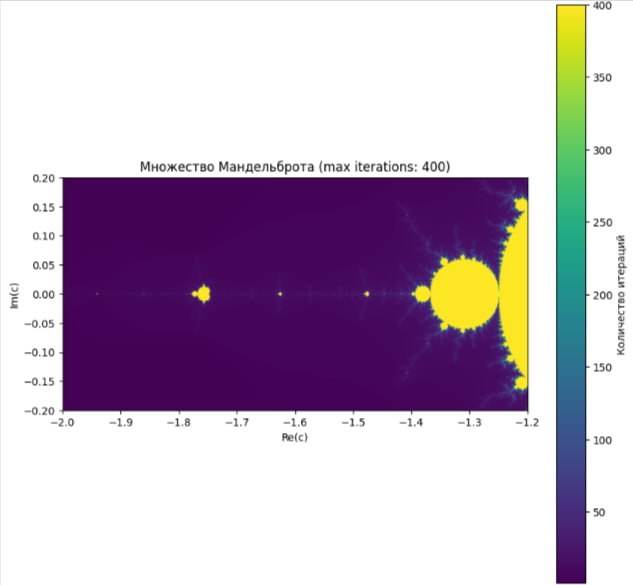
\includegraphics[width=\textwidth]{plots/M6.jpg}
        \caption{Максимальное приближение множества Мандельброта, 500~итераций }
    \end{subfigure}
\end{figure}